\newcommand{\qr}{../img/logo.png}
\newcommand{\dashboard}{../img/dashboard.png}


\newcolumntype{P}[1]{>{\centering\arraybackslash}p{#1}}
% Tabla 1
\begin{longtable}{|p{2.5cm}|p{8cm}|p{2cm}|p{1.5cm}|p{2cm}|}
    \hline
    \rowcolor{bleudefrance}
    \multicolumn{5}{|c|}{\color{aliceblue}\Large\textbf{HISTORIA DE USUARIO}}\\
    \hline\rowcolor{white} 
    \multicolumn{3}{|P{12cm}|}{Sistema Avanzado de Transcripción y Traducción
     Multilingue para Eventos Presenciales y Multimedia con
     Inteligencia Artificial} & \multicolumn{2}{c|}{ \raisebox{-\totalheight}{
\includegraphics[width=3cm]{\qr}}}\\
    \hline
    \rowcolor{bleudefrance} 
    \textbf{\color{aliceblue} ID} & \textbf{\color{aliceblue} Nombre corto de HU} & \textbf{\color{aliceblue} Prioridad} & \textbf{\color{aliceblue} PHU}& \textbf{\color{aliceblue}Estado}  \\
    \hline
    \rowcolor{lightgray} \textbf{ H.U.3} & \textbf{Interfaz de usuario} & \textbf{Baja} & \textbf{ }& \textbf{Completo} \\
    \hline
    \endfirsthead


    %Esto es para que la tabla se repita en cada pagina, cuando es muy larga
    \hline
    \rowcolor{bleudefrance}
    \multicolumn{5}{|c|}{\color{aliceblue}\Large\textbf{HISTORIA DE USUARIO}}\\
    \hline\rowcolor{white} 
    \multicolumn{3}{|P{12cm}|}{Sistema Avanzado de Transcripción y Traducción
     Multilingue para Eventos Presenciales y Multimedia con
     Inteligencia Artificial} & \multicolumn{2}{c|}{{
\includegraphics[width=3cm]{\qr}}}\\
    \hline
    \rowcolor{bleudefrance} 
    \textbf{\color{aliceblue} ID} & \textbf{\color{aliceblue} Nombre corto de HU} & \textbf{\color{aliceblue} Prioridad} & \textbf{\color{aliceblue} PHU}& \textbf{\color{aliceblue}Estado}  \\
    \hline
    \rowcolor{lightgray} \textbf{ H.U.3} & \textbf{Interfaz de usuario} & \textbf{Baja} & \textbf{ }& \textbf{Completo} \\
    \hline
    \endhead


    \cellcolor{bleudefrance}\textbf{\color{aliceblue} Como :} 
    & \multicolumn{4}{>{\columncolor{white}}l|}{Usuario} \\
    \hline
    \cellcolor{bleudefrance}\textbf{\color{aliceblue} Quiero :} 
    & \multicolumn{4}{>{\columncolor{white}}l|}{una interfaz amigable y
    fácil de usar} \\
    \hline
    \cellcolor{bleudefrance}\textbf{\color{aliceblue} Para :} 
    & \multicolumn{4}{>{\columncolor{white}}l|}{poder interactuar con el
    sistema sin complicaciones.} \\
    \hline
    \cellcolor{bleudefrance}\textbf{\color{aliceblue} Criterios de aplicación :} & \multicolumn{4}{>{\columncolor{white}}p{14cm}|}{
            \begin{itemize}
                \item Menu de navegación claro y accesible.
                \item Diseño responsivo para diferentes dispositivos.
                \item El sistema debe permitir al usuario ver su perfil y editar su información personal.
            \end{itemize}

            }\\    
    \hline
    \rowcolor{bleudefrance}
    \multicolumn{5}{|c|}{\textbf{\color{aliceblue} Conversación/Reglas (opcional)}}\\
    \hline
    \multicolumn{5}{|c|}{\textbf{ Aqui la descripcion}}\\
    \hline
    \rowcolor{bleudefrance}
    \multicolumn{5}{|c|}{\textbf{\color{aliceblue} Prototipo/Mockup (opcional)}}\\
    \hline
    \multicolumn{5}{|c|}{{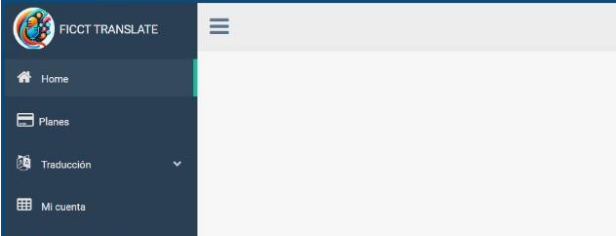
\includegraphics[width=13.4cm]{\dashboard}}}\\
    \hline
    \cellcolor{bleudefrance}\textbf{\color{aliceblue} Desarrollador:} 
    & \multicolumn{4}{|l|}{SAGREDO CORDOVA SIMON} \\
    \hline
    \rowcolor{bleudefrance}\multicolumn{5}{|c|}{ }\\
    \hline

\end{longtable}